\chapter{The Equivalence Principle, Tidal Forces, and the Metric}

Susskind begins almost exactly where Einstein began.  If general relativity is ultimately a theory of geometry, why not start with geometry?  Because Einstein did not.  He began with a simple physical fact that almost a child could understand: an accelerated frame and a gravitational field feel the same.  The lecture first turns that statement into equations in the slow-velocity, Newtonian regime.  Only after that does it pivot to space-time pictures, to the local distance formula, and finally to the tensor machinery needed to ask whether a metric is genuinely curved or merely written in awkward coordinates.

\section{Beginning with Einstein and the Equivalence Principle}

Susskind's opening move is methodological as much as physical.  He wants to begin with the simplest facts and squeeze consequences out of them, rather than beginning with a polished formalism and only later asking what it means.  The first of those facts is the equivalence principle.

\begin{definition}
For the purposes of this lecture, the equivalence principle says that gravity and acceleration are locally indistinguishable.  In a sufficiently small system, observed for a sufficiently short time, the effects of a gravitational field can be mimicked by going to an accelerated frame of reference.
\end{definition}

He immediately adds a second piece of staging.  At the beginning of the discussion we ignore special relativity.  We take
\begin{equation}
t'=t
\end{equation}
and think about motions slow enough that the speed of light may as well be infinite.  This is not a retreat from relativity.  It is a way of isolating the gravity--acceleration idea before combining it with Minkowski geometry.

The guiding question is therefore not yet, ``What is the geometry of curved space-time?''  It is simpler and more physical: if gravity and acceleration are in some sense the same thing, what does that actually mean when we write equations?

\section{The Elevator Formalized in Newtonian Coordinates}

To formalize the words, Susskind goes back to Einstein's elevator.  Let \(z\) be the vertical coordinate in a frame at rest with respect to the ground, and let \(z'\) be the vertical coordinate measured from the floor of the elevator.  If the floor of the elevator is at height \(L(t)\), then the same physical point has two coordinates related by
\begin{align}
z' &= z - L(t), \\
t' &= t, \\
x' &= x,
\end{align}
where the last equation simply says that the elevator is not sliding horizontally.  We may also assume that at \(t=0\) the two origins coincide.

This is a trivial coordinate transformation in one sense, since only the vertical coordinate changes in an interesting way.  But it is conceptually important, because the lecture is already training us to ask a general question: if we know the laws of physics in one coordinate system, how do they look in another?

\paragraph{Inertial frames.}
First take the harmless case.  Suppose the elevator moves with uniform velocity \(v\).  Then
\begin{equation}
L(t)=vt,
\end{equation}
so
\begin{equation}
z' = z-vt.
\end{equation}
Now consider the \(z\)-component of Newton's law:
\begin{equation}
F = m\ddot z.
\end{equation}
Differentiating the transformation twice with respect to time gives
\begin{equation}
\ddot z'=\ddot z,
\end{equation}
because the second derivative of \(vt\) vanishes.  Therefore Newton's law in the primed frame is
\begin{equation}
F=m\ddot z'.
\end{equation}
Nothing has happened.  That is precisely the Newtonian statement that inertial frames are equivalent, but Susskind wants us to notice the mechanism: a linear coordinate transformation leaves the form of the equation unchanged.

\begin{figure}[htbp]
\centering

\includegraphics[width=0.82\textwidth]{lecture_01_figure_02.png}
\caption{Newton's law specialized to the vertical coordinate}
\end{figure}

\paragraph{An accelerated frame.}
Now change only one ingredient.  Let the elevator accelerate uniformly upward.  Then
\begin{equation}
L(t)=\frac{1}{2}gt^2,
\end{equation}
so that
\begin{equation}
z' = z-\frac{1}{2}gt^2.
\end{equation}
Differentiating once and twice,
\begin{align}
\dot L &= gt, \\
\ddot L &= g,
\end{align}
and therefore
\begin{equation}
\ddot z'=\ddot z-g.
\end{equation}
At this point the lecture visibly checks the sign.  The point is worth preserving: the algebra is simple, but the interpretation depends on placing the extra term on the right side of the equation in the Newtonian way.  Rewriting,
\begin{align}
\ddot z &= \ddot z' + g, \\
F &= m(\ddot z' + g), \\
m\ddot z' &= F - mg.
\end{align}

Now something has happened.  In the accelerated frame there appears an extra force term, and it is proportional to the mass.  That is the crucial feature.  Gravity too produces a force proportional to \(m\), and because Newton's equation is \(F=ma\), the mass cancels from the motion.  The path of a freely falling object does not depend on its mass.  That is why the fictitious force in an accelerated elevator does not merely resemble gravity superficially.  It shares the decisive dynamical feature of a uniform gravitational field.

\section{Curvilinear Coordinates, Space-Time Pictures, and the Bending of Light}

Once the equations are on the board, Susskind shifts to pictures.  Every event has coordinates \((z,t)\) and also \((z',t')\), with \(t'=t\).  For the inertial transformation \(z'=z-vt\), the coordinate change is linear, and straight lines go to straight lines.

\begin{figure}[htbp]
\centering
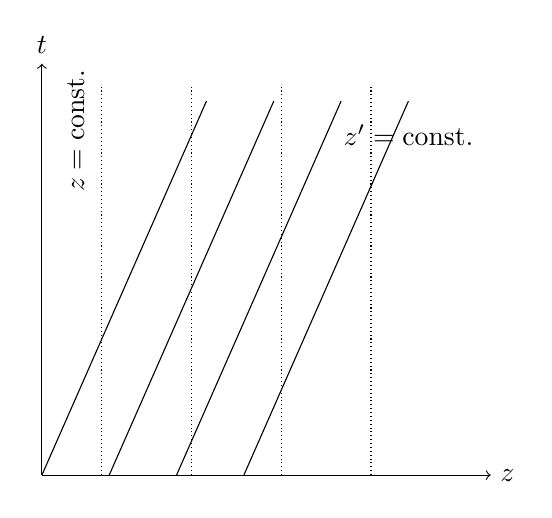
\begin{tikzpicture}[scale=0.95]
\draw[->] (0,0) -- (6,0) node[right] {$z$};
\draw[->] (0,0) -- (0,5.5) node[above] {$t$};
\foreach \a in {0.8,2.0,3.2,4.4} {
  \draw[densely dotted] (\a,0) -- (\a,5.2);
}
\foreach \b in {0.0,0.9,1.8,2.7} {
  \draw (\b,0) -- (\b+2.2,5.0);
}
\node at (4.9,4.55) {$z'=\mathrm{const.}$};
\node[rotate=90] at (0.45,4.6) {$z=\mathrm{const.}$};
\end{tikzpicture}
\caption{A linear coordinate transformation in the \(z\)-\(t\) plane}
\end{figure}

That is not a surprise.  Free particles move on straight worldlines in an inertial frame, and what is straight in one inertial frame had better remain straight in another.

The accelerated transformation,
\begin{equation}
z' = z-\frac{1}{2}gt^2,
\end{equation}
behaves differently.  The curves \(z'=\mathrm{const.}\) are now parabolas lying on their side.

\begin{figure}[htbp]
\centering
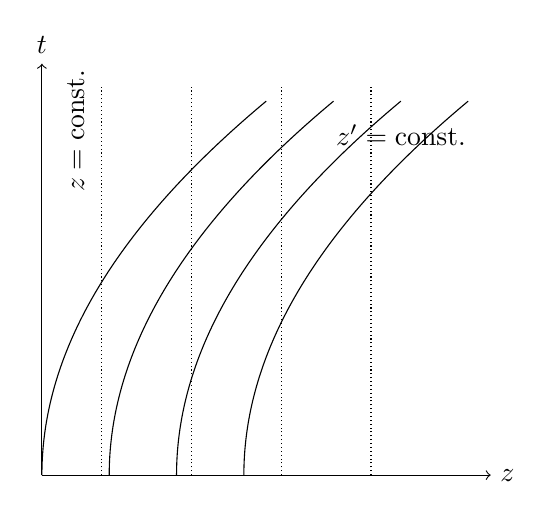
\begin{tikzpicture}[scale=0.95]
\draw[->] (0,0) -- (6,0) node[right] {$z$};
\draw[->] (0,0) -- (0,5.5) node[above] {$t$};
\foreach \a in {0.8,2.0,3.2,4.4} {
  \draw[densely dotted] (\a,0) -- (\a,5.2);
}
\foreach \b in {0.0,0.9,1.8,2.7} {
  \draw[smooth,domain=0:5,samples=80] plot ({0.12*\x*\x+\b},{\x});
}
\node at (4.8,4.55) {$z'=\mathrm{const.}$};
\node[rotate=90] at (0.45,4.6) {$z=\mathrm{const.}$};
\end{tikzpicture}
\caption{An accelerated coordinate system in the \(z\)-\(t\) plane}
\end{figure}

This is the first geometrical payoff of the earlier algebra.  A nonlinear coordinate transformation of space-time produces effective gravitational forces, and correspondingly it also produces curvilinear coordinate lines.  Einstein saw very early that gravity had something to do with curvilinear coordinate transformations of space-time.

Now comes the famous question: what does gravity do to light?  Before Einstein, many physicists would simply have said, nothing.  Light moves in straight lines; gravity acts on masses.  But the equivalence principle says more.

Take a light ray emitted horizontally at \(t=0\).  In the unprimed frame, where there is no gravitational field, it satisfies
\begin{equation}
x=ct, \qquad z=0.
\end{equation}
In the accelerated frame we use
\begin{equation}
z = z' + \frac{1}{2}gt^2,
\end{equation}
so the same light ray satisfies
\begin{equation}
z' + \frac{1}{2}gt^2 = 0, \qquad x=ct.
\end{equation}
Eliminating \(t\) gives the trajectory in the \((x,z')\)-plane:
\begin{equation}
z' = -\frac{g}{2c^2}x^2.
\end{equation}
So the beam is curved in the accelerated frame.

\begin{figure}[htbp]
\centering
\begin{tikzpicture}[scale=1.0]
\draw[->] (0,0) -- (5.8,0) node[right] {$x$};
\draw[->] (0,-2.3) -- (0,1.0) node[above] {$z'$};
\draw[densely dashed] (0,0) -- (5.3,0);
\draw[thick,smooth,domain=0:5.2,samples=100] plot (\x,{-0.08*\x*\x});
\node at (3.8,-1.5) {$z'=-\dfrac{g}{2c^2}x^2$};
\end{tikzpicture}
\caption{The light ray in the accelerated frame}
\end{figure}

One may say, and Susskind does say, that this only proves that acceleration makes light look bent.  Einstein's point was sharper.  If gravity and acceleration are locally equivalent in the physically relevant sense, then gravity must bend light.

\section{Real Gravity, Fake Gravity, and Tidal Forces}

But now the lecture deliberately slows down.  If an accelerated frame can create a gravitational field, does that mean every gravitational field is merely a coordinate artifact?  Not at all.

A genuine gravitational field, such as the field of the Earth or the Sun, points radially inward.  In a small freely falling laboratory one can make gravity disappear locally.  But there is no global coordinate transformation that will remove an inward-pointing radial field everywhere at once.  What disappears at one place reappears somewhere else.

The physical reason is tidal force.  Consider Susskind's favorite example, the \(2{,}000\)-mile man.  If he falls feet first toward a gravitating body, his feet are pulled more strongly than his head.  He is stretched.  If he falls sideways, different parts of him are pulled in different directions and he is squeezed.  These effects are not matters of notation.  Being stretched or squashed is an invariant physical fact.

The lecture widens the point further.  By choosing more complicated curvilinear coordinates one can manufacture much more complicated apparent gravitational fields than the simple uniform field of the elevator.  One can accelerate upward while oscillating in the horizontal direction.  One can use polar coordinates and discover centrifugal and Coriolis forces.  In those coordinates the motion may look as though some gravitational field is pushing outward or sideways.  The important question is therefore not whether a field \emph{looks} gravitational.  The important question is whether it leaves tidal effects on freely falling matter.

\subsection{Question \& Answer}

Can gravity always be transformed away?

Only locally.  A uniform effective field, the sort produced in a sufficiently small freely falling laboratory, can be removed by an appropriate choice of coordinates.  A genuine gravitational field cannot be removed globally, because tidal forces remain.

In Newtonian language the diagnostic is simple.  Drop a freely falling object, or if one wants a more dramatic picture, drop a crystal.  Ask whether it develops distorting stresses: stretching in one direction, squeezing in another.  If no freely falling body ever develops such stresses, then the field is fictitious and can be blamed on coordinates.  If such stresses are present, then there is a real gravitational field.

This is why the equivalence principle has to be stated carefully.  It does not say that gravity is globally identical to acceleration.  It says that for a sufficiently small system, small enough that the field does not vary appreciably across it, the two are indistinguishable to that accuracy.  The residue that cannot be transformed away is tidal force.

\section{From the Minkowski Interval to the Metric Tensor}

At this point Susskind says, in effect, let us take a rest from gravity.  We come back to special relativity only for one reason: Minkowski space already taught us that space-time carries geometry.

For neighboring events in one space and one time direction, the invariant interval may be written as
\begin{equation}
d\tau^2 = dt^2 - dx^2.
\end{equation}
Some authors instead write
\begin{equation}
ds^2 = dx^2 - dt^2,
\end{equation}
which differs only by a sign convention.  If one keeps \(c\) explicit, one may insert factors of \(1/c^2\) and then absorb them by redefining the coordinate.  The main point is that special relativity gives us an invariant local notion of distance in space-time.

Einstein recognized that the question we have just been asking about gravity is mathematically close to a question already studied by Gauss and Riemann: given the local distance formula of a geometry, how do we know whether the geometry is really flat?

In ordinary Euclidean space with Cartesian coordinates, the answer is just Pythagoras:
\begin{equation}
ds^2 = \sum_i (dx^i)^2 = \delta_{mn}\,dx^m dx^n.
\end{equation}
But on a curved surface, or even on a flat surface described by curved coordinates, the distance between arbitrary separated points is a complicated notion.  One may define it as the length of a shortest path, like a taut string stretched across a bumpy surface, and then one must know the geometry everywhere in between.  The distance between neighboring points is much simpler.  That local distance is exactly what the metric encodes.

So if we place arbitrary coordinates \(x^1,x^2,\dots\) on a surface, the most general local distance formula takes the quadratic form
\begin{equation}
ds^2 = \sum_{m,n} g_{mn}(x)\,dx^m dx^n.
\end{equation}
The coefficients \(g_{mn}(x)\) are the components of the metric tensor in that coordinate system.

The sphere gives the simplest example.  If \(\theta\) is measured from the north pole, then
\begin{equation}
ds^2 = R^2\bigl(d\theta^2 + \sin^2\theta\,d\phi^2\bigr).
\end{equation}
If instead \(\theta\) is measured from the equator, then the same geometry is written as
\begin{equation}
ds^2 = R^2\bigl(d\theta^2 + \cos^2\theta\,d\phi^2\bigr).
\end{equation}
The convention changes, but the lesson does not: the coefficient of \(d\phi^2\) depends on position.

\begin{figure}[htbp]
\centering

\includegraphics[width=0.82\textwidth]{lecture_01_figure_03.png}
\caption{General line element over a local curved coordinate patch}
\end{figure}

The board at this point is especially instructive.  The formula is not written in isolation.  It sits beside local axes labeled \(x^1\) and \(x^2\), above a curved coordinate net drawn on a patch, and below a small curvilinear-grid sketch.  The visual logic is that the metric is the quadratic form attached to a chosen coordinate chart.

\begin{figure}[htbp]
\centering
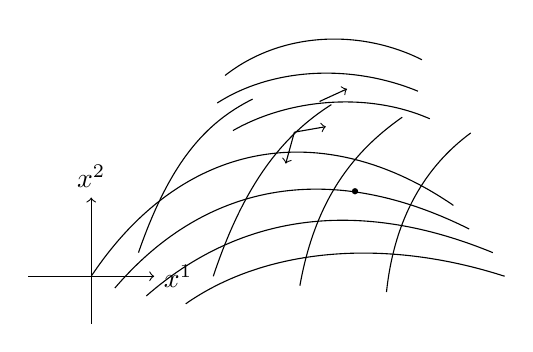
\begin{tikzpicture}[scale=1.0]
\draw[->] (-0.8,0) -- (0.8,0) node[right] {$x^1$};
\draw[->] (0,-0.6) -- (0,1.0) node[above] {$x^2$};

\begin{scope}[shift={(2.8,2.2)}]
\draw[smooth] (-1.1,0.35) .. controls (-0.4,0.9) and (0.6,0.95) .. (1.4,0.55);
\draw[smooth] (-1.2,0.0) .. controls (-0.5,0.45) and (0.5,0.5) .. (1.35,0.15);
\draw[smooth] (-1.0,-0.35) .. controls (-0.3,0.05) and (0.7,0.15) .. (1.5,-0.2);
\draw[->] (0.1,0.02) -- (0.45,0.18);
\end{scope}

\draw[smooth] (0.0,0.0) .. controls (1.2,1.8) and (3.0,2.0) .. (4.6,0.9);
\draw[smooth] (0.3,-0.15) .. controls (1.5,1.25) and (3.1,1.45) .. (4.8,0.6);
\draw[smooth] (0.7,-0.25) .. controls (1.9,0.8) and (3.4,1.0) .. (5.1,0.3);
\draw[smooth] (1.2,-0.35) .. controls (2.2,0.35) and (3.7,0.5) .. (5.25,0.0);

\draw[smooth] (0.6,0.3) .. controls (1.0,1.45) and (1.45,1.95) .. (2.05,2.25);
\draw[smooth] (1.55,0.0) .. controls (1.95,1.2) and (2.45,1.8) .. (3.05,2.18);
\draw[smooth] (2.65,-0.12) .. controls (2.85,1.0) and (3.35,1.6) .. (3.95,2.02);
\draw[smooth] (3.75,-0.2) .. controls (3.85,0.75) and (4.25,1.4) .. (4.82,1.82);

\fill (3.35,1.08) circle (0.04);
\draw[->] (2.58,1.83) -- (2.98,1.90);
\draw[->] (2.58,1.83) -- (2.47,1.43);
\end{tikzpicture}
\caption{A schematic redraw of the local curved coordinate patch associated with the metric formula}
\end{figure}

\begin{figure}[htbp]
\centering

\includegraphics[width=0.82\textwidth]{lecture_01_figure_04.png}
\caption{One metric tensor in a chosen coordinate chart}
\end{figure}

Susskind now introduces an image that will carry a great deal of the rest of the course: imagine building a geometry out of little sticks, little differential pieces whose lengths are fixed by the metric.  Perhaps they can be laid down flat on a plane without stretching; then the geometry is flat.  Or perhaps they fit together on a sphere but cannot be flattened onto a plane; then the geometry is intrinsically curved.

\section{Intrinsic Geometry and the Flatness Question}

The next step is to sharpen the question.  Suppose I hand you one set of coordinates and one metric tensor \(g_{mn}(x)\).  Then, in effect, I have told you the distance between every pair of neighboring points.  Can you tell whether the geometry is flat?

\subsection{Question \& Answer}

Given one metric tensor, how do we test flatness?

Not by staring at a single point.  At a point every smooth surface looks flat.  One can even choose coordinates that diagonalize the metric at a point.  That does not decide the global question.  The real question is whether there exists a coordinate transformation to new coordinates \(X^m\) in which the interval becomes everywhere
\begin{equation}
ds^2 = \delta_{mn}\,dX^m dX^n.
\end{equation}
If such coordinates exist everywhere, the space is flat.  If no such coordinates exist, the space is curved.

This is the precise geometric analogue of the earlier physics problem.  There the question was whether a gravitational field could be removed by a coordinate transformation.  Here the question is whether the ``curvy character'' of the metric can be removed by a coordinate transformation.

\begin{figure}[htbp]
\centering

\includegraphics[width=0.82\textwidth]{lecture_01_figure_05.png}
\caption{Pointing to the position-dependent metric factor}
\end{figure}

Susskind's pointing gesture matters here.  The ``curvy character'' is not the differentials \(dx^m\) themselves; it is the coefficient \(g_{mn}(x)\), the fact that the metric components vary with position.

There is also a local subtlety that the lecture takes time to emphasize.  The metric formula is a formula for neighboring points, not for arbitrary macroscopic separations.  That is why tests such as comparing a small circumference with \(2\pi r\) are delicate in differential form: for an infinitesimal circle the deviation from the Euclidean value appears only at higher order.  Small enough pieces always look flat to first approximation; geometrically, they are approximated by the tangent space.

This local flatness does not mean the whole geometry is flat.  It only means that curvature cannot be diagnosed at a single point by zeroth-order inspection.

The lecture then turns to the distinction between intrinsic and extrinsic geometry.  A sheet of paper can be folded, wrinkled, or creased in the surrounding three-dimensional space, and yet its intrinsic geometry may remain the geometry of a flat plane.  The relevant distances are distances \emph{along} the surface, not straight-line distances through the embedding space.  That is why a crease is not the same thing as intrinsic curvature.  The metric itself may remain continuous even when some of its derivatives do not.

\begin{figure}[htbp]
\centering

\includegraphics[width=0.82\textwidth]{lecture_01_figure_06.png}
\caption{Folded surface sketch and local coordinate patch}
\end{figure}

\begin{figure}[htbp]
\centering
\begin{tikzpicture}[scale=0.92]
\begin{scope}
\draw[smooth] (-3.1,1.7) .. controls (-2.2,2.5) and (-1.1,2.1) .. (-0.4,1.7)
.. controls (0.2,1.3) and (0.9,2.45) .. (1.5,1.75)
.. controls (2.1,1.1) and (2.8,1.25) .. (3.3,1.45);
\draw[smooth] (-3.0,0.75) .. controls (-1.6,0.95) and (0.3,0.9) .. (3.25,0.8);
\foreach \x in {-2.5,-1.5,-0.2,1.1,2.5} {
  \draw[->] (\x,0.5) -- (\x,-1.3);
}
\end{scope}

\begin{scope}[xshift=8.0cm]
\draw[->] (-0.9,0) -- (0.9,0) node[right] {$x^1$};
\draw[->] (0,-0.7) -- (0,1.0) node[above] {$x^2$};

\draw[smooth] (0.0,0.0) .. controls (0.8,1.15) and (2.0,1.25) .. (3.15,0.55);
\draw[smooth] (0.3,-0.2) .. controls (1.1,0.75) and (2.2,0.88) .. (3.35,0.25);
\draw[smooth] (0.8,-0.35) .. controls (1.5,0.28) and (2.5,0.4) .. (3.5,-0.02);

\draw[smooth] (0.55,-0.1) .. controls (0.85,0.7) and (1.15,1.0) .. (1.65,1.25);
\draw[smooth] (1.45,-0.25) .. controls (1.7,0.55) and (2.05,0.88) .. (2.55,1.15);
\draw[smooth] (2.45,-0.35) .. controls (2.6,0.35) and (2.95,0.7) .. (3.35,0.98);

\fill (2.2,0.55) circle (0.04);
\end{scope}
\end{tikzpicture}
\caption{A schematic intrinsic-versus-extrinsic picture: folding changes the embedding, not the local distance relations on the surface}
\end{figure}

This is where the lecture states the deeper lesson explicitly.  The relation between tidal force and curvature is not just a loose analogy.  In general relativity, genuine gravity is diagnosed by curvature, and flatness means vanishing curvature.  The machinery for proving that comes later, but the target has now come into focus.

\section{Tensor Analysis as the Next Tool}

Once the problem is stated this way, tensor analysis no longer looks ornamental.  It is forced on us.  If the question is whether a given metric can be simplified by a coordinate change, then the first thing we must know is how the metric transforms when coordinates change.

Susskind therefore introduces two coordinate systems, \(x^m\) and \(y^m\), avoiding the notation \(x'^m\) simply because it becomes unreadable once indices and primes pile up together.  The coordinates are assumed to be smooth functions of one another.

The differential coordinate transformation is just the chain rule:
\begin{equation}
dy^m = \frac{\partial y^m}{\partial x^p}\,dx^p.
\end{equation}
Because the \(dx^m\) are the components of an infinitesimal displacement vector, this equation becomes the model transformation law for a contravariant vector:
\begin{equation}
V'^m = \frac{\partial y^m}{\partial x^p}\,V^p.
\end{equation}
An object with components transforming this way is called contravariant.

A different kind of vector appears when we begin with a scalar \(s(x)\).  Its gradient is
\begin{equation}
W_m = \frac{\partial s}{\partial x^m}.
\end{equation}
Applying the chain rule again,
\begin{equation}
W'_m = \frac{\partial x^p}{\partial y^m}\,W_p.
\end{equation}
This is the transformation law for a covariant vector.  The lecture insists on the conceptual point: at this stage contravariant and covariant vectors are simply different kinds of objects, distinguished by how they transform.

The pattern for higher-rank tensors is built from products.  If
\begin{equation}
T^{mn}=V^mU^n,
\end{equation}
then each upper index picks up its own Jacobian factor:
\begin{equation}
T'^{mn} = \frac{\partial y^m}{\partial x^p}\frac{\partial y^n}{\partial x^q}T^{pq}.
\end{equation}
Likewise, for a tensor with two lower indices,
\begin{equation}
T'_{mn} = \frac{\partial x^p}{\partial y^m}\frac{\partial x^q}{\partial y^n}T_{pq}.
\end{equation}

At this point Susskind pauses over notation.  Tensor analysis is annoying mainly because of the indices, not because the ideas are deep.  Einstein's summation convention removes much of the clutter: once an index is repeated in a term, we understand it to be summed over, without writing the summation sign explicitly.

The metric now returns as the crucial example:
\begin{equation}
ds^2 = g_{mn}(x)\,dx^m dx^n.
\end{equation}
To rewrite the same interval in the \(y\)-coordinates, one substitutes
\begin{equation}
dx^m = \frac{\partial x^m}{\partial y^p}\,dy^p.
\end{equation}
Carrying this through shows that the metric transforms as a tensor with two covariant indices.

The lecture stops just there.  It does not yet complete the full transformation law in detail, and it does not yet derive the curvature tensor.  Instead it leaves us with the right hard question: given the transformation property of \(g_{mn}\), can we or can we not find a coordinate transformation that turns it into \(\delta_{mn}\)?  That is the flatness question.  In the next lecture it becomes the doorway to curvature, and therefore to gravity itself.

\section{Summary}

The argument of the lecture unfolds in a very definite order.  We first formalize the equivalence principle in Newtonian language: an accelerated elevator produces an effective uniform gravitational field, and the mass-proportional extra force term explains why it really does mimic gravity.  We then translate that algebra into geometry of coordinates in space-time, and from there extract Einstein's first striking consequence: gravity bends light.

But the lecture does not stop with that triumph.  It immediately raises the obstruction.  Real gravity cannot be transformed away globally because tidal forces remain.  That obstruction is then recast as a geometric problem: given a local distance formula, how do we know whether the geometry is really flat?  The metric tensor is introduced as the object that answers the local distance question, and tensor analysis is introduced as the machinery needed to study how that object changes under coordinate transformations.  The chapter therefore ends exactly where the lecture ends: with the metric identified as a rank-two covariant tensor, and with the flatness problem now posed in fully mathematical form.